% This is samplepaper.tex, a sample chapter demonstrating the
% LLNCS macro package for Springer Computer Science proceedings;
% Version 2.21 of 2022/01/12
%
\documentclass[runningheads]{llncs}
%
\usepackage[T1]{fontenc}
% T1 fonts will be used to generate the final print and online PDFs,
% so please use T1 fonts in your manuscript whenever possible.
% Other font encondings may result in incorrect characters.
%
\usepackage{graphicx}
% Used for displaying a sample figure. If possible, figure files should
% be included in EPS format.
%
% If you use the hyperref package, please uncomment the following two lines
% to display URLs in blue roman font according to Springer's eBook style:
%\usepackage{color}
%\renewcommand\UrlFont{\color{blue}\rmfamily}
%\urlstyle{rm}
%
\usepackage{cite}
\usepackage{amsmath,amssymb,amsfonts}
\usepackage{algorithmic}
\usepackage[ruled,vlined]{algorithm2e}
\usepackage{textcomp}
\usepackage{xcolor}
\usepackage{booktabs}
\usepackage{bbding}
\usepackage{multirow}
\usepackage{subfigure}
\usepackage[utf8]{inputenc}
\usepackage{authblk}
\usepackage{float}
\usepackage[misc]{ifsym}
\usepackage[table]{xcolor}


\begin{document}

%
\title{Collaborative Enhanced Attention for Speech Emotion Recognition Based on Multimodal Acoustic Information Fusion}
%
\titlerunning{Collaborative Enhanced Attention for SER}
% If the paper title is too long for the running head, you can set
% an abbreviated paper title here
%
\author{Ping Lin\inst{1} \and
Can Bu\inst{1} \and
Yongming Huang\inst{1}\textsuperscript{(\Letter)}}
%
\authorrunning{P. Lin et al.}
% First names are abbreviated in the running head.
% If there are more than two authors, 'et al.' is used.
%
\institute{School of Automation, Southeast University, Nanjing, China\\ 
\email{\texttt{huang\_ym@seu.edu.cn}}
%\url{http://www.springer.com/gp/computer-science/lncs} \and
%ABC Institute, Rupert-Karls-University Heidelberg, Heidelberg, Germany\\
%\email{\{abc,lncs\}@uni-heidelberg.de}
}
%
\maketitle              % typeset the header of the contribution
%
\begin{abstract}
Speech emotion recognition (SER) aims to infer human emotions based on speech information. Effectively and comprehensively combining the various pieces of information in the audio for accurate judgment remains a significant challenge. In this paper, we propose a novel SER network based on a Collaborative Enhanced Attention (CEA) mechanism. Initially, we apply wavelet transform to translate the raw speech into the frequency domain, obtaining log spectrograms. We then use EfficientNet and Mamba to extract acoustic features. Finally, CEA and Co-attention are used to fuse these features with high-level acoustic information embedded through the WavLM model. The CEA is specifically designed to refine the acoustic information within WavLM features by accentuating different aspects of the signal, thereby enhancing the feature representation from multiple perspectives. We evaluate our method on the IEMOCAP dataset, where the weighted accuracy and unweighted accuracy improved by 4.96\% and 4.71\%, respectively. Our code is available on https://github.com/Chara2001/CEA-SER.git.

\keywords{Speech emotion recognition \and Collaborative enhanced attention \and Wavelet transform \and Multimodal fusion.}
\end{abstract}
%
%
%
\section{Introduction}
\label{sec:intro}

Speech emotion recognition (SER) has become an important component of human-computer interaction. The emotional modality in speech is applied in some spoken dialogue systems, such as call center conversations, in-vehicle driving systems, and others \cite{b1}. Despite the emergence of some multimodal methods that have achieved high recognition accuracy in emotion recognition \cite{b10,b11,b12}, these models are not widely applied, and there may be redundancy and interference of information between different modalities. In contrast, the speech modality is easier to obtain, so we focus on the research of SER tasks.

The SER method mainly consists of two stages: feature extraction and feature classification. In the feature extraction stage, Al-Ali et al.\cite{b2} enhanced the accuracy of emotion recognition by stacking spectral centroid, pitch frequency, and spectral roll-off on the spectrogram; Yuan et al.\cite{b3} designed DTNet to disentangle emotional and acoustic features, extracting more discriminative emotional features; Chen et al.\cite{b4} proposed a deformable speech transformer called DST to adaptively discover and focus on valuable embedded information in speech; Zhang et al.\cite{b6} introduced an autoencoder with emotional embedding to extract deep emotional features. In the feature classification stage, Ong et al.\cite{b5} proposed an improved multi-scale visual transformer (MViTv2) to effectively model interactions between labels in spatiotemporal structures; Hashemi et al.\cite{b7} used frame-based Vision Transformer (ViT) and parallel Convolutional Neural Network (CNN) to learn both global and local features in SER; Ye et al.\cite{b8} introduced a time-aware bi-directional multi-scale network (TIM-Net) to learn multi-scale contextual emotional representations from various temporal scales. Although these methods have improved the accuracy of SER, they only use one type of speech information, which inevitably leads to the loss of other speech feature information.

To address this issue, Zou et al.\cite{b19} proposed a SER method based on multi-level acoustic information, which simultaneously uses three acoustic features: Mel-Frequency Cepstral Coefficients (MFCC), log spectrogram, and features extracted by the Wav2Vec2 model. He et al.\cite{b14} employed a cross-attention transformer to process dual-source inputs based on these three acoustic features. Pan et al.\cite{b9} replaced the Wav2Vec2 model with the Hubert model and proposed a Global Perception Feature Representation Network (GFRN-SEA) for speech emotion analysis. These studies all introduced different attention mechanisms to process the extracted features. However, since general-purpose models like Wav2Vec2 may extract features that contain not only emotional information but also a lot of other information, this could affect the model's emotional recognition performance. Therefore, a mechanism is needed that can collaborate with different feature information and the advanced acoustic information embedded in the WavLM model, in order to enhance its emotional information.

In this study, we propose a SER method based on the Collaborative Enhancement Attention (CEA) module for multimodal acoustic information fusion.  In this method, we select three types of features as network inputs: logarithmic spectrogram, MFCC, and large-model speech features. However, unlike traditional methods, we apply the wavelet transform to convert the original audio signal into the frequency domain. This transformation effectively captures the time-varying characteristics of speech signals, thereby enhancing the ability to extract emotional features.  Next, we employ EfficientNet for further feature extraction from the spectrogram. Although the MFCC better align with human auditory characteristics, they often overlook temporal dependencies during processing. To address this, we introduce the Mamba\cite{b17} model, a linear temporal analysis model based on the Selective State Space Model (SSM), which effectively captures both short-term and long-term dependencies, significantly improving the model's emotion recognition performance.  Additionally, we utilize the advanced large-scale speech model WavLM\cite{b13} to directly extract features from the raw audio signal. In the feature fusion stage, we designed the CEA mechanism, which dynamically learns attention weights to effectively enhance emotion-related information in the WavLM features (WLM). The CEA mechanism also applies weighted adjustments to each frame of the signal using spectrogram and MFCC features, compensating for time-frequency information that may be lost during training. Finally, the processed features are concatenated and fed into a classifier composed of three fully connected layers to achieve emotion classification.

Our main contributions are summarized as follows:
\begin{itemize}
\item We propose an SER network that integrates logarithmic spectrogram, MFCC, and self-supervised large model features, with EfficientNet, Mamba, and WavLM employed respectively to further extract emotional information from these three features.  
\item We innovatively apply the Continuous Wavelet Transform (CWT) to process the original audio, effectively capturing the emotional characteristics of short-term speech in the frequency domain.  
\item We design a novel Collaborative Enhancement Attention mechanism, which enhances emotional information in features through dual pathways and compensates for missing information, enabling the network to perform more comprehensive emotion recognition.
\end{itemize}

\section{Proposed method}
This section introduces the proposed SER method. In the following subsections, we will provide a detailed description of the feature extraction module and the proposed collaborative enhancement attention mechanism.

\subsection{Overall Architecture}

The overall SER method is shown in Figure \ref{mainnet}. We represent the MFCC, log-spectrogram, and WavLM obtained from the same audio segment as \(x_m\in \mathbb{R}^{D_m}\), \(x_s\in \mathbb{R}^{T_{s}\times D_s}\), and \(x_w\in \mathbb{R}^{T_{w}\times 1}\), respectively. This method first uses EfficientNet\cite{b18} to extract frequency features from the log-spectrogram obtained via wavelet transform. The Mamba module is then used to extract timbral and temporal features from the MFCC. Additionally, WavLM, a large pre-trained model, is employed to directly extract feature sequences from the raw audio signal, without the need for fine-tuning. Next, the extracted MFCC features and spectrogram features are passed through linear layers for transformation, in preparation for fusion with WLM. The three features are further processed using co-attention\cite{b19} mechanisms and collaborative enhancement attention mechanisms to capture dependencies between different parts of the features, thus enhancing the model's ability to learn emotional features. Finally, the MFCC features, spectrogram features, and the features processed by the two attention mechanisms are concatenated and fed into a classifier composed of three fully connected layers for emotion recognition.
\begin{figure*}[htbp]
\centering

\includegraphics[width=1.0\linewidth]{mainnet_colorline_2pt.jpg}
\caption{The main framework of our proposed method}
\label{mainnet}
\end{figure*}

\subsection{MFCC processing}

MFCC is a core feature in speech signal processing, designed to simulate the nonlinear frequency perception characteristics of the human auditory system. We process the MFCC sequence through the Mamba module, with a state sequence factor of 64, a local convolution kernel width of 4, and a block expansion factor of 2. As shown in Figure 1, the Mamba module first obtains the MFCC input embedding through linear projection. Then, a convolution operation is applied before the Selective State Space Model (Selective SSM). Afterward, the linearly projected state after SSM processing is multiplied by the activated linear projection, and finally passed through another layer of linear projection to generate the output. The calculation process of SSM is as follows:
\begin{equation}
h'(t)=Ah(t)+Bx(t), 
\end{equation}
\begin{equation}
y(t)=Ch(t), 
\end{equation}
here, \( h(t) \) represents the hidden state at the current time step, \( x(t) \) is the input at the current time step, \( h'(t) \) is the updated hidden state, \( y(t) \) is the output at the current time step, and \( A \), \( B \), and \( C \) are learnable parameters.

\begin{figure*}[htbp]
\centering
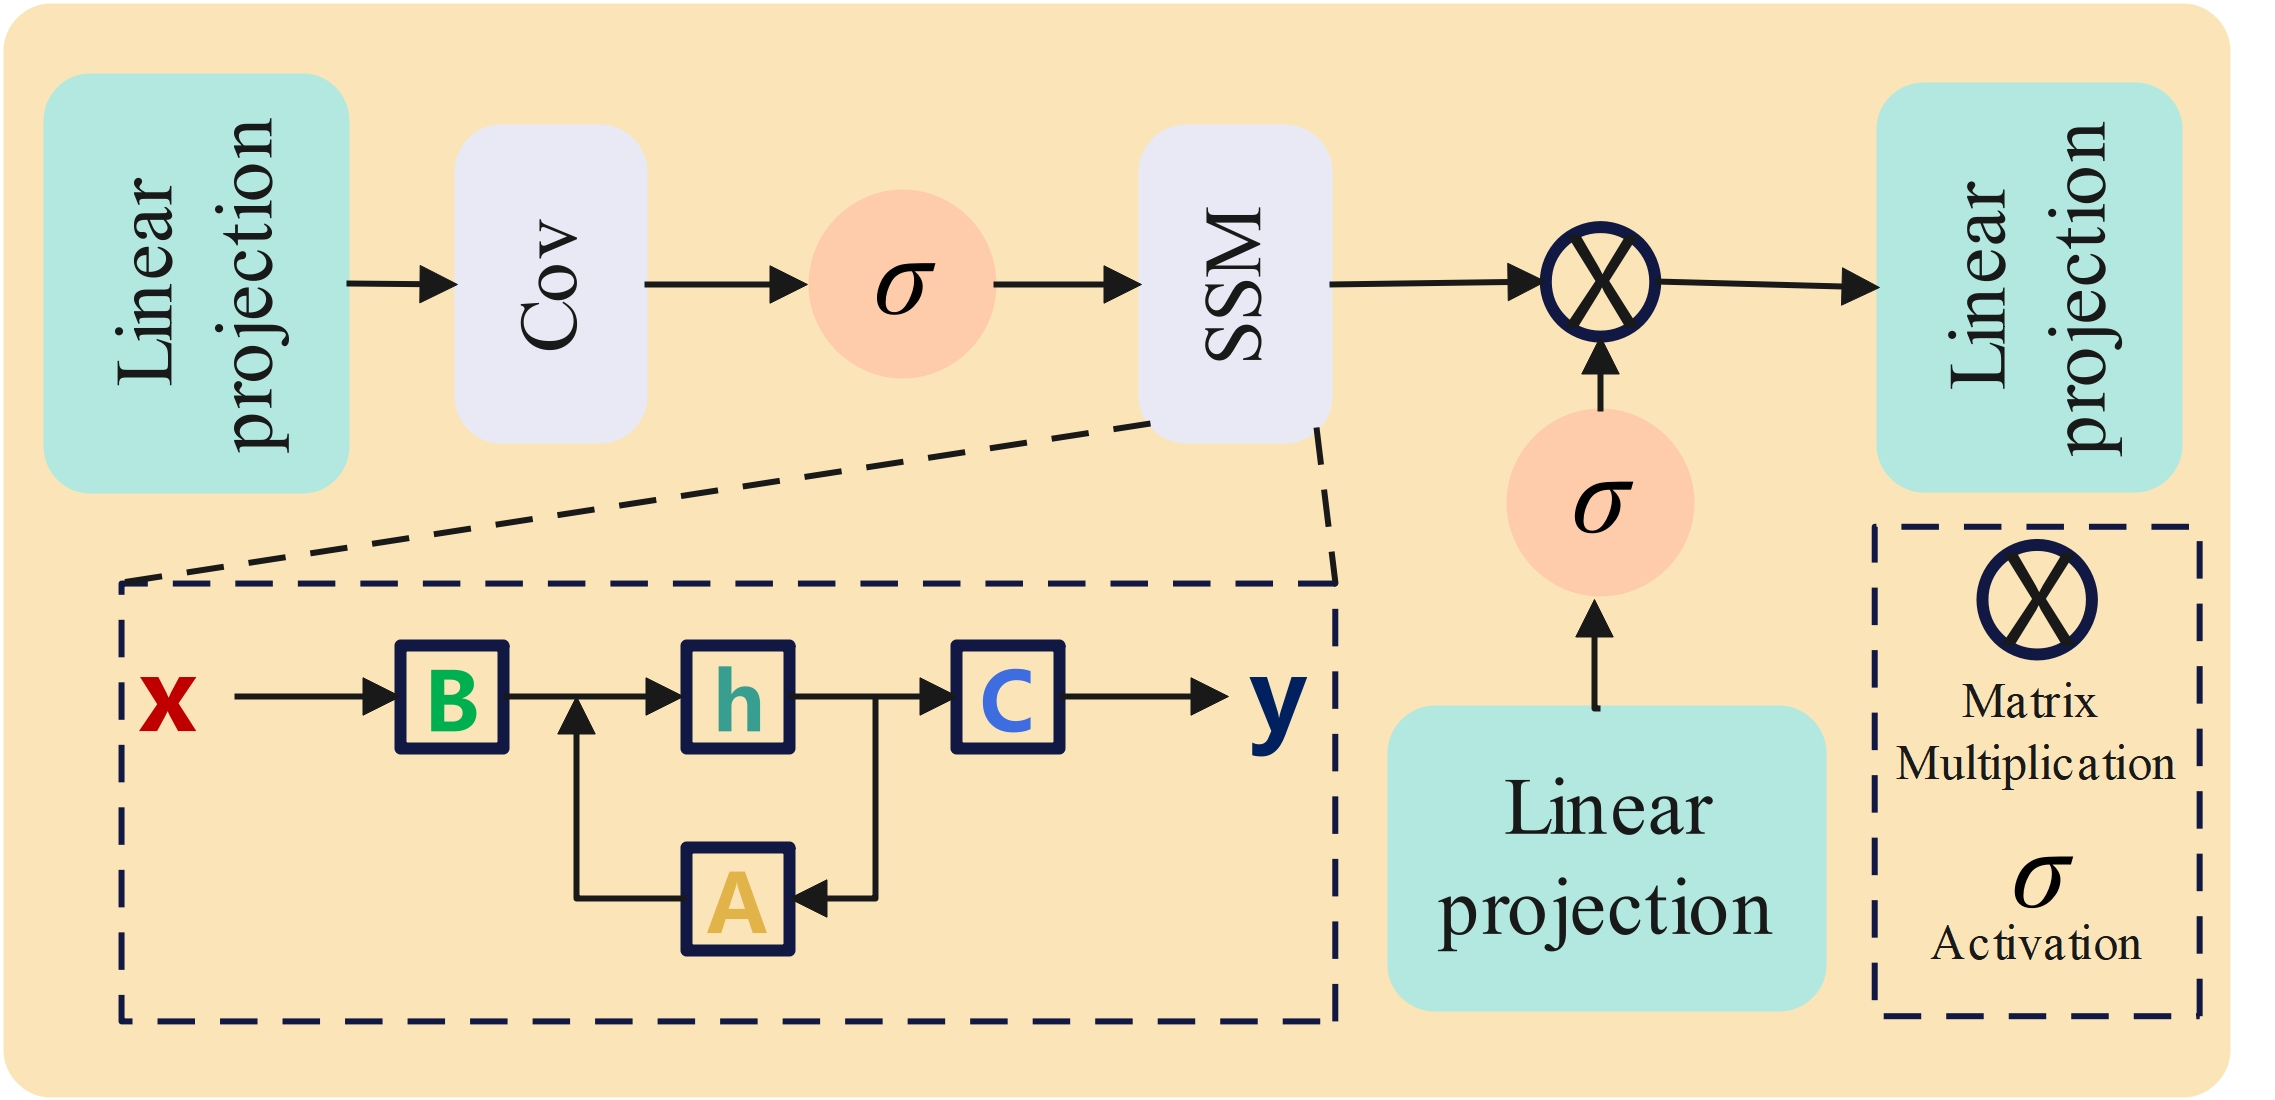
\includegraphics[width=1.0\linewidth]{mamba_new.jpg}
\caption{The structure of selective SSM}
\label{figure_SSM}
\end{figure*}

Selective SSM expands the model's capability by introducing a selective mechanism, allowing it to better capture the complex dynamic behaviors in MFCC and extract features that influence these dynamics. At the same time, selective SSM focuses only on the states that are important for emotion recognition, significantly reducing the computational load and improving computational efficiency. The structure of SSM is shown in Figure \ref{figure_SSM}. The processed vectors are then fed into a linear layer, with Rectified Linear Unit (ReLU) as the activation function and a dropout rate of 0.1, in order to obtain:
\begin{equation}
x^{'}_{m}=f_{m}(Mamba(x_m)),
\end{equation}
where \(x^{'}_{m}\in \mathbb{R}^{D'_m}\), \(f_{m}\) represents the linear transformation and activation operation applied to the output features of Mamba.

\subsection{Log-spectrogram processing}

SER tasks require extracting emotion-related features such as pitch, speech rate, and volume variations from speech signals. Thanks to the time-frequency localization property of wavelet transform, this method can more accurately capture short-term fluctuation features of speech signals, thereby improving the accuracy of emotion recognition. For emotional speech with rapid and instantaneous changes, features extracted by Fourier transform may not effectively reflect the dynamic changes in emotion. Therefore, this study uses CWT to obtain the log-spectrogram of the original speech, as shown in the following formula:
\begin{equation}
W(a,b)=\int_{+\infty}^{-\infty}x(t)\cdot \psi_{a,b}^*(t) \, dt, 
\end{equation}
where W(a,b) is the wavelet transform coefficient, x(t) is the original signal, $\psi_{a,b}^*(t) = (1/\sqrt a) \cdot \psi((t - b)/a)$ is the scaled (scale) and translated (translation) mother wavelet function, $a$ is the scale parameter, which controls the frequency resolution, $b$ is the translation parameter, which controls the time resolution,  \(\psi^*\) represents the complex conjugate of the mother wavelet. In this paper, we use the Morlet wavelet as the mother wavelet. 

\begin{figure*}[htbp]
\centering
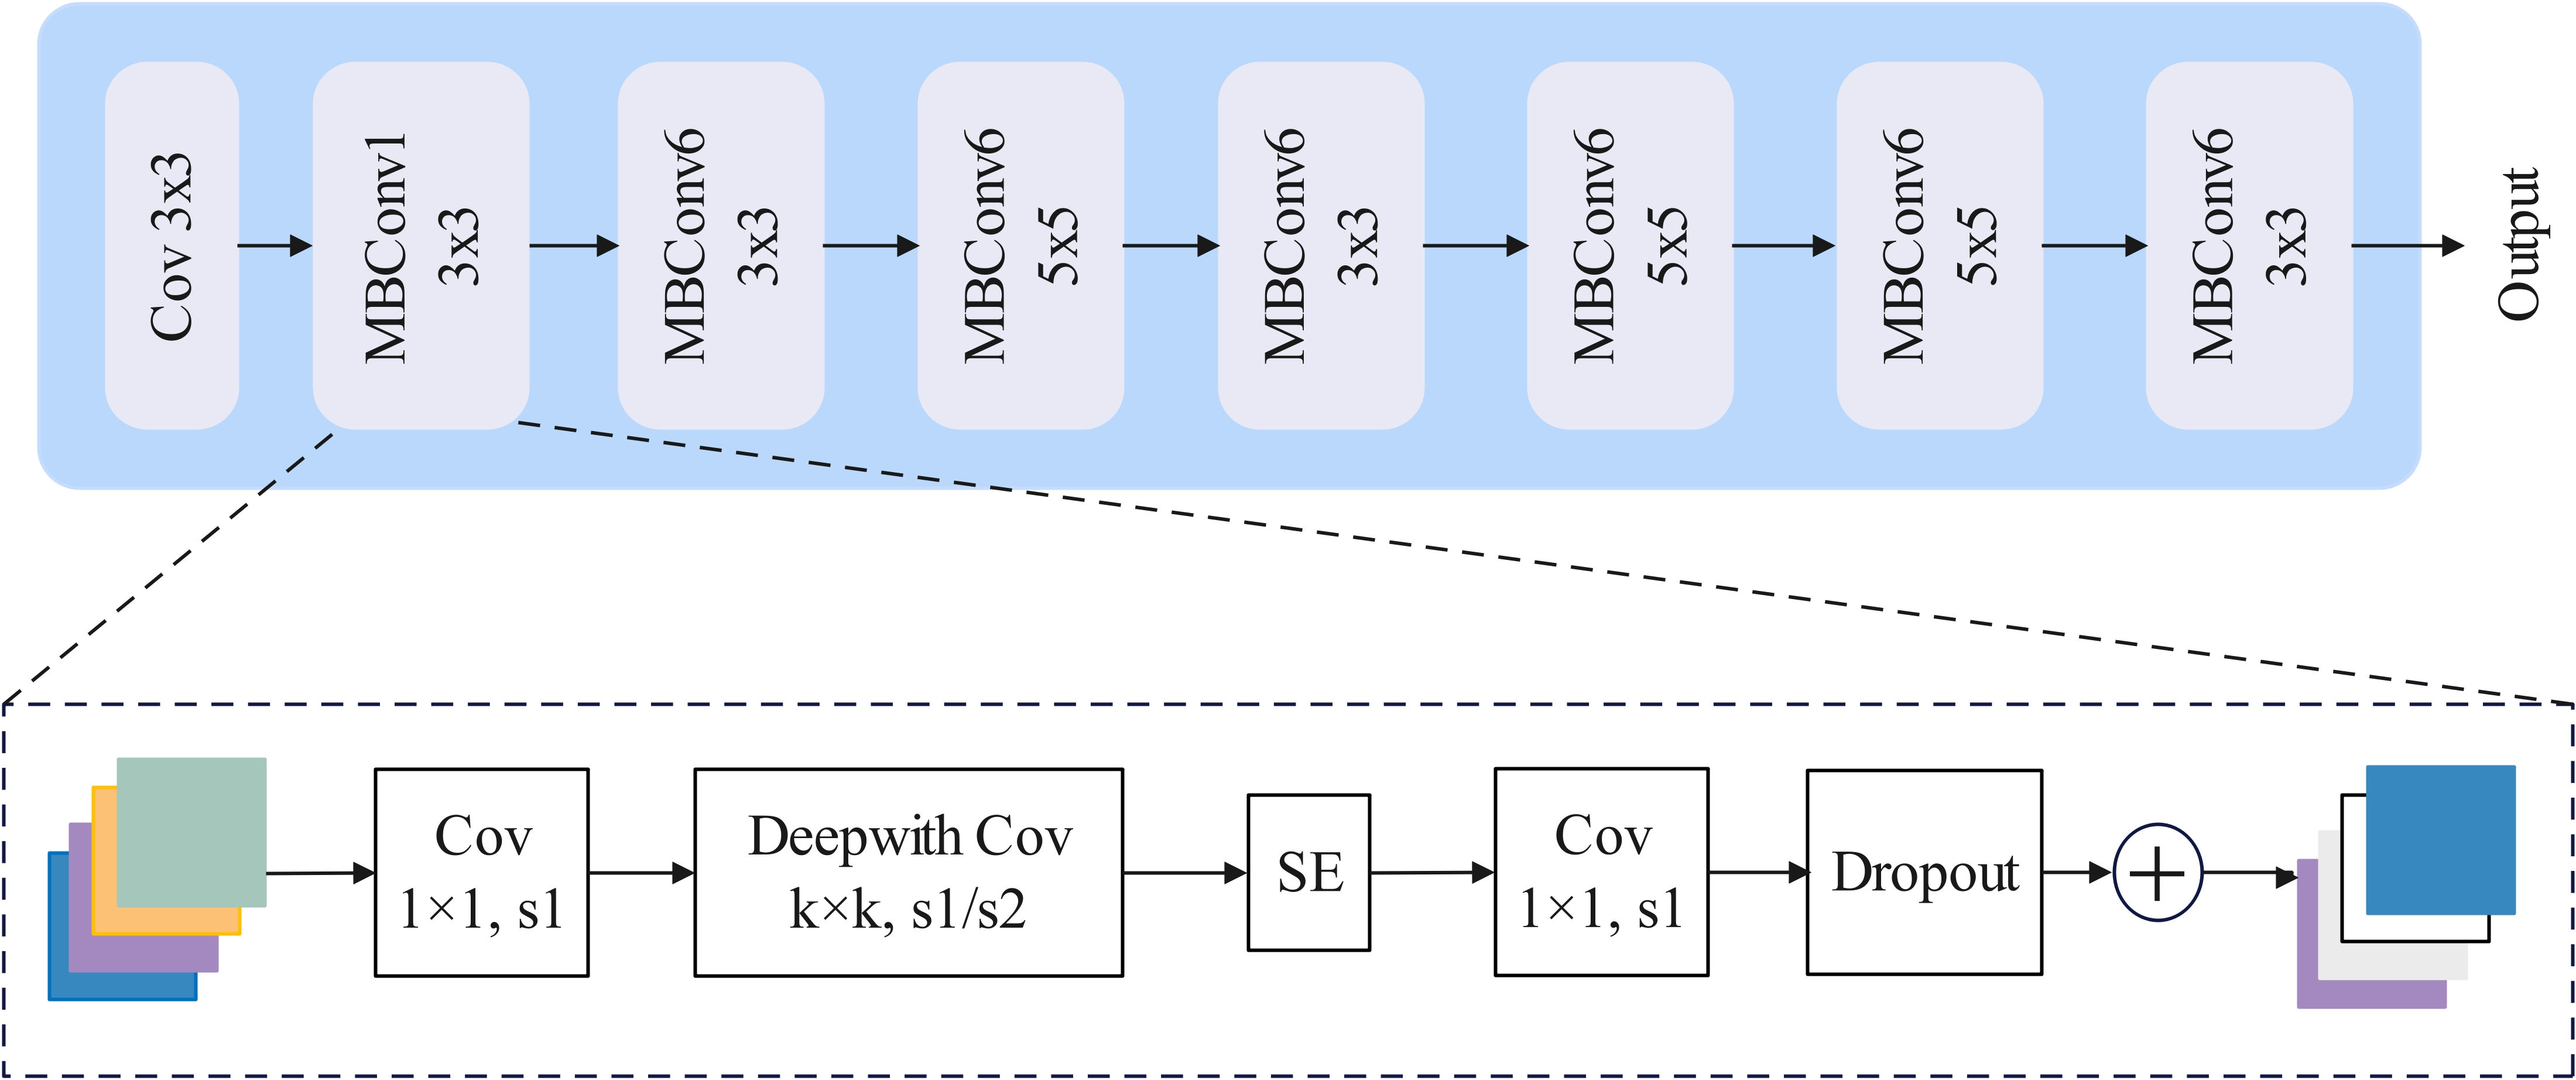
\includegraphics[width=1.0\linewidth]{efficientnet.jpg}
\caption{The structure of EfficientNet}
\label{figure_efficient}
\end{figure*}
Next, we encode the spectrogram features using the pre-trained EfficientNet (network structure detailed in Figure \ref{figure_efficient}). EfficientNet is an efficient CNN architecture proposed by the Google Brain team, which achieves better performance with fewer parameters. Its core module is based on the inverted residual structure from MobileNetV2, combined with depthwise separable convolution, effectively reducing computational complexity. We then follow the same processing steps as in MFCC, ultimately obtaining:
\begin{equation}
x^{'}_{s}=f_{s}(EfficientNet(x_s)),
\end{equation}
where \(x^{'}_{s}\in \mathbb{R}^{D'_s}\), \(f_{s}\) represents the linear transformation and activation operation applied to the output features of EfficientNet.

\subsection{WavLM Feature Processing}
WavLM is a self-supervised speech representation learning model proposed by Microsoft Research. Through pretraining on large-scale unlabeled speech data, it can extract speech features that contain rich fine-grained semantic and acoustic information. The core idea is to simulate the multi-level characteristics of human speech understanding, capturing both acoustic details and semantic context in speech signals. Due to the advanced structure of WavLM, we use WavLM to directly extract features from the raw audio. The raw audio is first processed by the WavLM preprocessor, then input into the WavLM model to extract a series of raw WavLM features:
\begin{equation}
x^{'}_{w}=f_{w}(WavLM(x_w)),
\end{equation}
where \(x^{'}_{w}\in \mathbb{R}^{{T'_w}\times {D'_w}}\), \(f_{w}\) represents the linear transformation and activation operation applied to the WLM.

\begin{figure}[htbp]
\centering
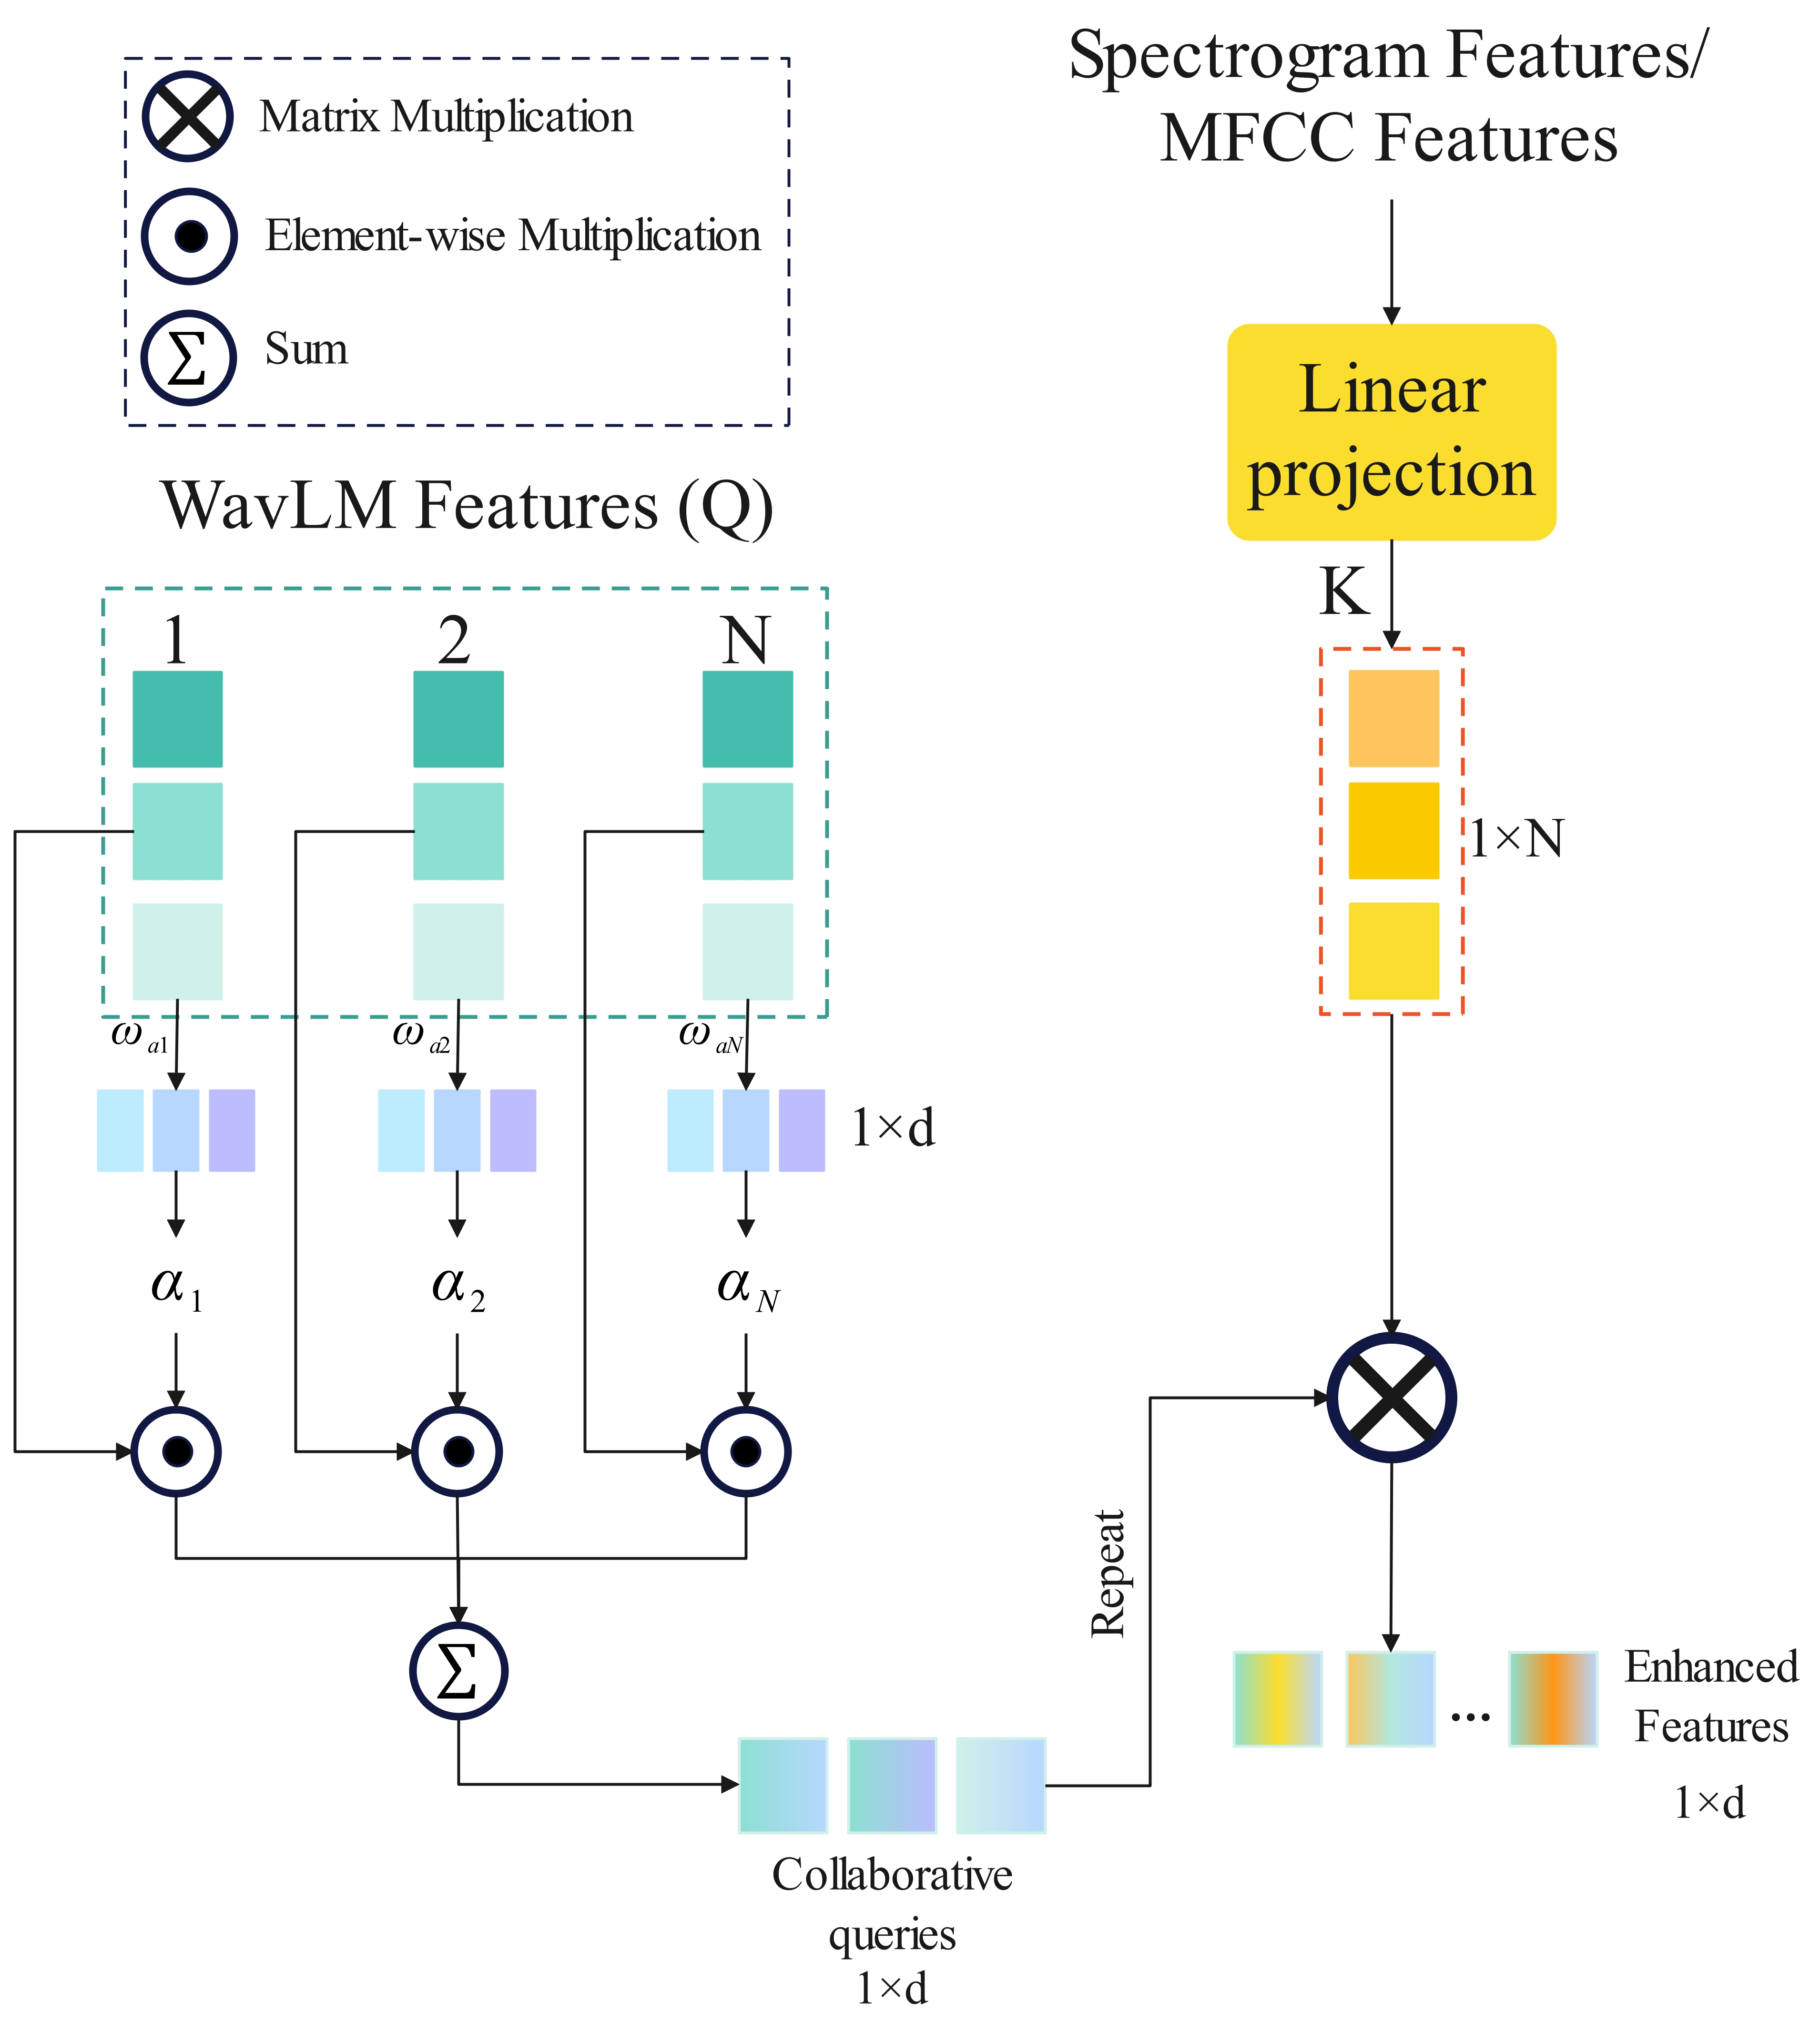
\includegraphics[width=1.0\linewidth]{attention_right.jpg}
\caption{Collaborative-Enhanced-Attention module}
\label{CEA}
\end{figure}
\subsection{Collaborative-Enhanced-Attention Based Fusion}
Related researches indicate that weighting the different frames of features extracted by large models can provide guidance for SER tasks\cite{b9},\cite{b19}. We use WavLM as a feature extractor for the raw audio input, where the output of WavLM represents the input audio signal (typically raw audio waveform) at multiple time steps. In addition to emotion-related information in the audio, these representations also contain information useful for other downstream tasks. We refer\cite{b19} to previous work and incorporate a co-attention mechanism into the network. However, we believe that simply using co-attention alone cannot effectively assist in the fusion of the three types of features and cannot fully extract the emotional information from the WLM. In this context, we propose CEA for the SER task, as shown in the computational flow in Figure \ref{CEA}. In CEA, we use \( x'_w \) to represent Q, \( x'_s\) to represent \( K_s \), and  \(x'_m \)  to represent \( K_m \). \( K_m \) and \( K_s \) will be used to collaborate with Q, considering both frequency and time perspectives. First, \( Q \), as the vector to be collaborated and enhanced, is multiplied by a learnable weight matrix to learn the enhanced attention weights, thus generating the enhanced attention vector \( \alpha \in \mathbb{R}^{D'_w} \):
\begin{equation}
\alpha=Q{\omega}_a/\sqrt{d}.
\end{equation}

Then, based on the learned attention weights, the features in \( Q \) are enhanced, allowing the model to more effectively focus on emotion-related information, resulting in a single collaborative queries \(q\in \mathbb{R}^{D'_w}\):
\begin{equation}
q=\sum_{i=1}^{n}\alpha_{i} \cdot Q_i.
\end{equation}

Since the collaborative queries \( q \) obtained after this process is derived by summing all the frames of \( Q \), it clearly loses some information along the sequence dimension. Therefore, we use \( K_m \) and \( K_s \) to perform collaboration along the sequence dimension on the stacked \( Q' \) matrix formed by repeating the \( q \) vector, thereby supplementing the lost information. In this process, \( K_s \) collaborates with \( Q' \) in the frequency domain to obtain \( x_{sw}\in \mathbb{R}^{1\times {D'_w}} \), while \( K_m \) collaborates with \( Q' \) in the temporal domain to obtain \( x_{mw}\in \mathbb{R}^{1\times {D'_w}} \):
\begin{equation}
x_{sw}=K_{s} Q',
\end{equation}
\begin{equation}
x_{mw}=K_{m} Q'.
\end{equation}

We concatenate \( x_{mw} \) and \( x_{sw} \), and input them into a linear layer to obtain:
\begin{equation}
x_{wc}=f(x_{sw}\oplus x_{mw}),
\end{equation}
where \(x_{wc}\in \mathbb{R}^{D_{wc}}\).

Finally, we concatenate the MFCC features, logarithmic spectrogram features, and the WavLM features processed by both the co-attention and collaborative enhancement attention mechanisms. The final emotion prediction output is:
\begin{equation}
\hat{y}=f(x^{'}_{m}\oplus x^{'}_{s}\oplus x^{''}_{w}\oplus x_{wc}), 
\end{equation}
where \( x''_w \) represents the WLM features processed by the co-attention mechanism.
%The algorithmic process of CEA is represented as follows:
%\begin{algorithm}
%\renewcommand{\algorithmicrequire}{\textbf{Input:}}
%\renewcommand{\algorithmicensure}{\textbf{Output:}}
%\caption{CEA's computation process}
%\begin{algorithmic}
%    \REQUIRE $K, Q$                  %输入条件
%    \ENSURE $out$       %输出
%    \STATE $q_w=Qw_a$
%    \STATE $A=q_w/\sqrt{d}$
%    \STATE $G=sum(AQ,dim=1)$
%    \STATE $Q'=repeat(G)$
%    \STATE $out=kQ'$
%    \RETURN out
%\end{algorithmic}
%\end{algorithm}
\subsection{Loss Function}
We use cross-entropy as the loss function for emotion classification, and our objective is as follows:
\begin{equation}
min L=L_{ce}(y-\hat{y}).
\end{equation}


\section{Experiments}
\subsection{Dataset}
We validate the proposed method on the Interactive Emotional Dyadic Motion Capture (IEMOCAP)\cite{b20} dataset. This dataset is widely used in various emotion recognition tasks and consists of 10 actors, with 5 different sessions, each performed by two native English-speaking actors (one male and one female). Following previous work\cite{b19}, \cite{b16}, we merge the $``$excited$"$ and $``$happy$"$ categories into a single $``$happy$"$ category. We consider a total of 5531 voice samples from four emotional categories: anger, sadness, happiness, and neutral. To compare with baseline methods, we test our model using 10-fold leave-one-speaker cross-validation and evaluate performance using the commonly used weighted accuracy (WA) and unweighted accuracy (UA) metrics.

\subsection{Experiment Setup}
The raw audio in the dataset has a sampling rate of 16 kHz. In our experiments, each audio sample is segmented into several 3-second clips. If the segment length is shorter than 3 seconds, we pad it with zeros. We use the librosa library to extract 40-dimensional MFCCs from the raw audio segments. For frequency-domain transformation, we apply CWT using the morlet wavelet as the mother wavelet, with a frequency resolution set to 200. The power spectrum of the signal is obtained by calculating the square of the wavelet coefficients' magnitude. We then apply a logarithmic transformation to the power spectrum, converting it into a logarithmic scale spectrogram, with 300 time steps set. WavLM features are extracted from the pre-trained WavLM model, corresponding to the output of the last hidden layer of the WavLM model.

The optimizer used for model training is AdamW, with a learning rate set to \( 3\times 10^{-5} \). The batch size for training is 32, and early stopping is configured with a patience of 10 epochs. 
\subsection{Results and Comparison}

\begin{table}[h]
\centering
\caption{Compare with the state-of-the-art models evaluated on the IEMOCAP dataset, where 'L' denotes the logarithmic spectrogram, 'M' represents the MFCC, and 'A' signifies the audio waveform.} % 添加标题
\label{main_exp} % 设置标签
\begin{tabular}{lllcc} 
\hline % 一条横线
\textbf{Reference} & \textbf{Model} & \textbf{Features} & \textbf{WA}(\%) & \textbf{UA}(\%) \\
\hline % 一条横线
Zou et al.\cite{b19} & Co-attention &  L + M + A  & 71.64 & 72.70 \\
He et al.\cite{b14} & SMW\_CAT & L + M + A  & 73.80 & 74.25 \\
Liu et al.\cite{b15} & DCW + TsPA & M + A  & 73.18 & 74.26 \\
Jiao et al.\cite{b16} & MFHCA & M + A  & 74.24 & 74.57 \\
Pan et al.\cite{b9} & GFRN-SEA & L + M + A  & 75.29 & 75.57 \\
\hline % 一条横线
 \rowcolor[HTML]{EFEFEF} & \textbf{CEA(Ours)} & L + M + A & \textbf{76.60} & \textbf{77.41} \\
 &\textbf{$\uparrow$} Improvement      &   & \textcolor[HTML]{346B96}{\textbf{$\uparrow$ 1.31}}    &   \textcolor[HTML]{346B96}{\textbf{$\uparrow$ 1.84}} \\
\hline % 一条横线
\hline % 一条横线
Zou et al.\cite{b19} & Co-attention &  L + M + A  & 69.80 & 71.05 \\
Tarantino et al.\cite{b21} & IS09 - classification & A  & 68.10 & 63.80 \\
Li et al.\cite{b22} &GLNN & A  & 71.83 & 65.39 \\
\hline % 一条横线
 \rowcolor[HTML]{EFEFEF}  & \textbf{CEA(Ours)} & L + M + A & \textbf{74.46} & \textbf{74.27} \\
  &\textbf{$\uparrow$} Improvement      &   & \textcolor[HTML]{346B96}{\textbf{$\uparrow$ 2.63}}    &   \textcolor[HTML]{346B96}{\textbf{$\uparrow$ 8.88}} \\
\hline % 一条横线
\end{tabular}
% 标题和标签写在这里也可以
\end{table}
Table \ref{main_exp} compares our method with baseline methods in terms of weighted accuracy (WA) and unweighted accuracy (UA) using both 10-fold leave-one-speaker-out and 5-fold leave-one-session-out methods. The methods in references \cite{b19}, \cite{b14}, \cite{b15}, \cite{b16}, \cite{b9} adopt the 10-fold leave-one-speaker-out approach, while those in references \cite{b19}, \cite{b21}, \cite{b22} adopt the 5-fold leave-one-session-out method. 
SMW\_CAT employs a co-attention mechanism with a Cross-Attention Transformer (CAT) to process dual-source inputs. GFRN-SEA designs a new convolutional module to extract information from log spectrograms and MFCCs and utilizes multi-layer cross-attention to fuse three types of acoustic information.  
Reference \cite{b15} reduces one type of acoustic information, designs a Discriminative Channel Weighting (DCW) module to weight MFCC, and introduces Two-stream Pooling Attention (TsPA) to fuse two features. MFHCA also reduces one type of acoustic information, designs a Multi-Spatial Fusion module (MF) to extract features from the spectrogram, and uses hierarchical attention for feature fusion. IS09-classification explores whether SER can benefit from Transformer-based self-attention and global windowing. GLNN establishes a speech graph based on feature similarity and introduces a novel graph neural network architecture that employs an LSTM aggregator and weighted pooling.  Experimental results show that our method achieves the best performance, with WA reaching 76.60\% and UA reaching 77.41\% in the 10-fold leave-one-speaker-out method. In the 5-fold leave-one-session-out method, WA reaches 74.46\% and UA reaches 74.27\%. These results demonstrate that leveraging wavelet transform for log-spectrogram extraction, using the Mamba module for MFCC feature extraction, and employing the CEA module for feature fusion significantly enhance SER performance.
\subsection{Ablation Study}

\begin{figure}[htbp]
\centering
\subfigure[Final features w/o CEA]
%\subfloat[Final features w/o CEA]
{
    \begin{minipage}[b]{0.8\linewidth}
        \centering
        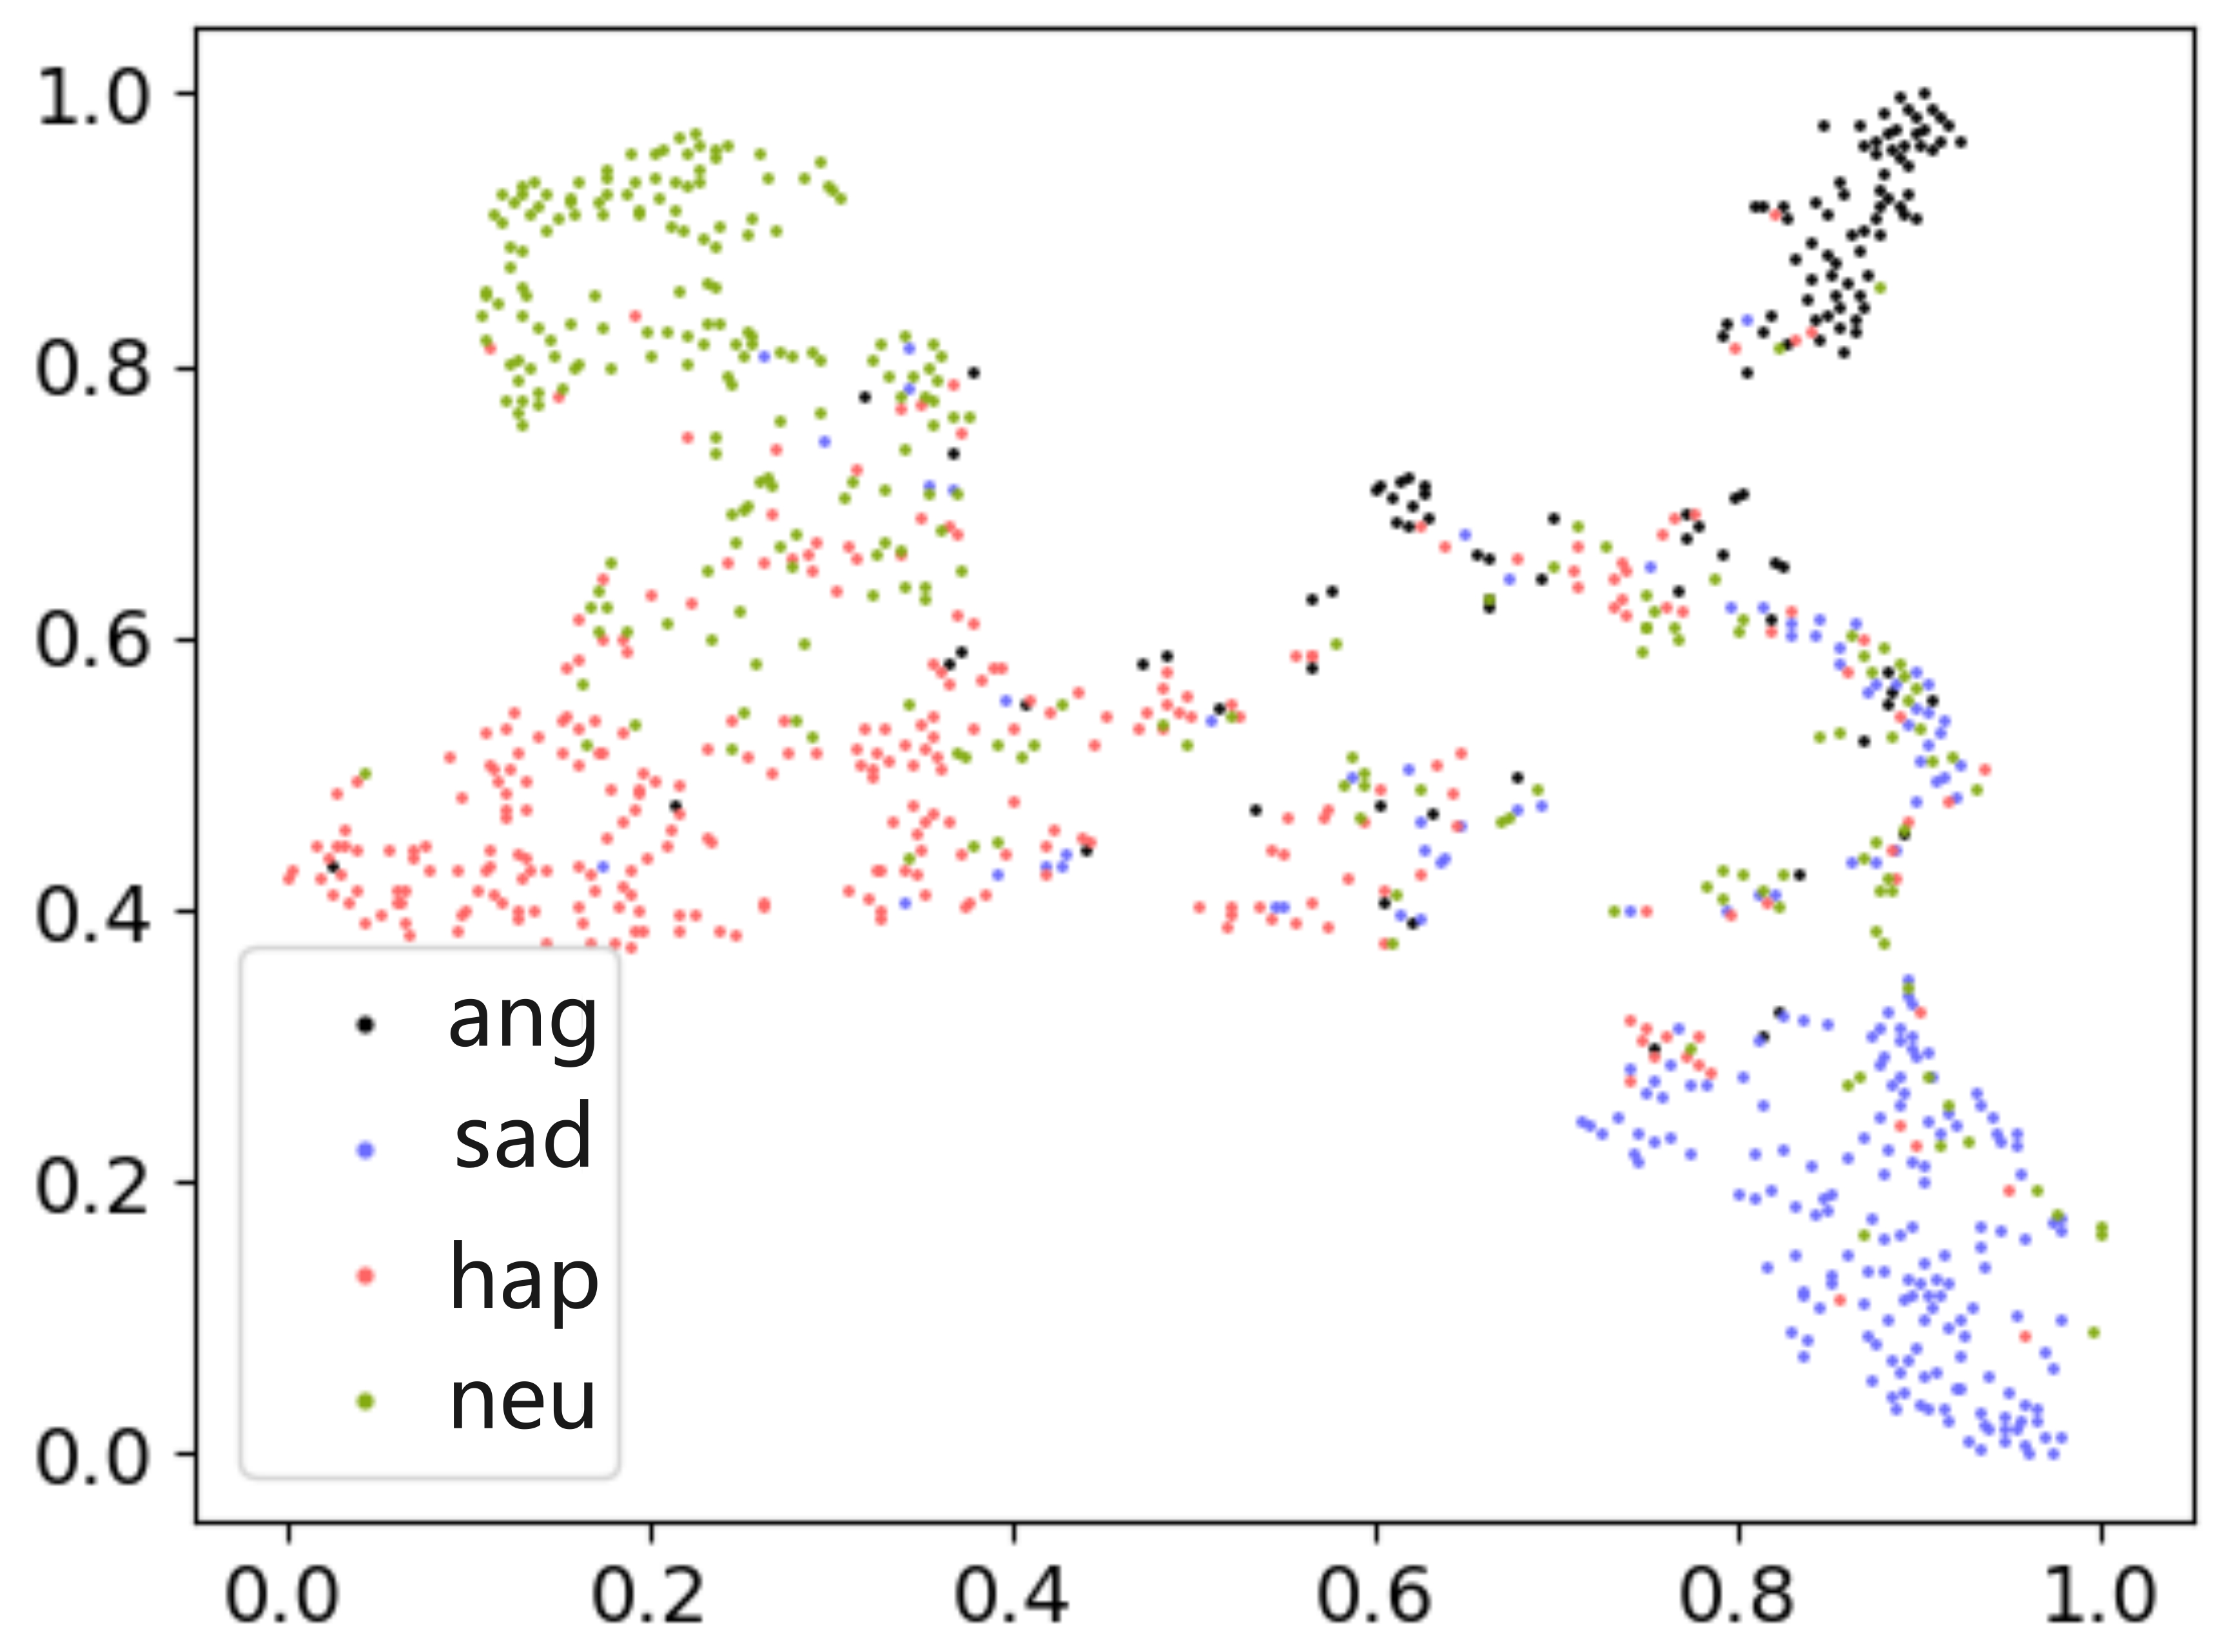
\includegraphics[width=0.8\linewidth]{withoutCEA_0_2_Fagain.jpg}
    \end{minipage}
}
\subfigure[Final features w/ CEA]
%\subfloat[Final features w/ CEA]
{
 	\begin{minipage}[b]{0.8\linewidth}
        \centering
        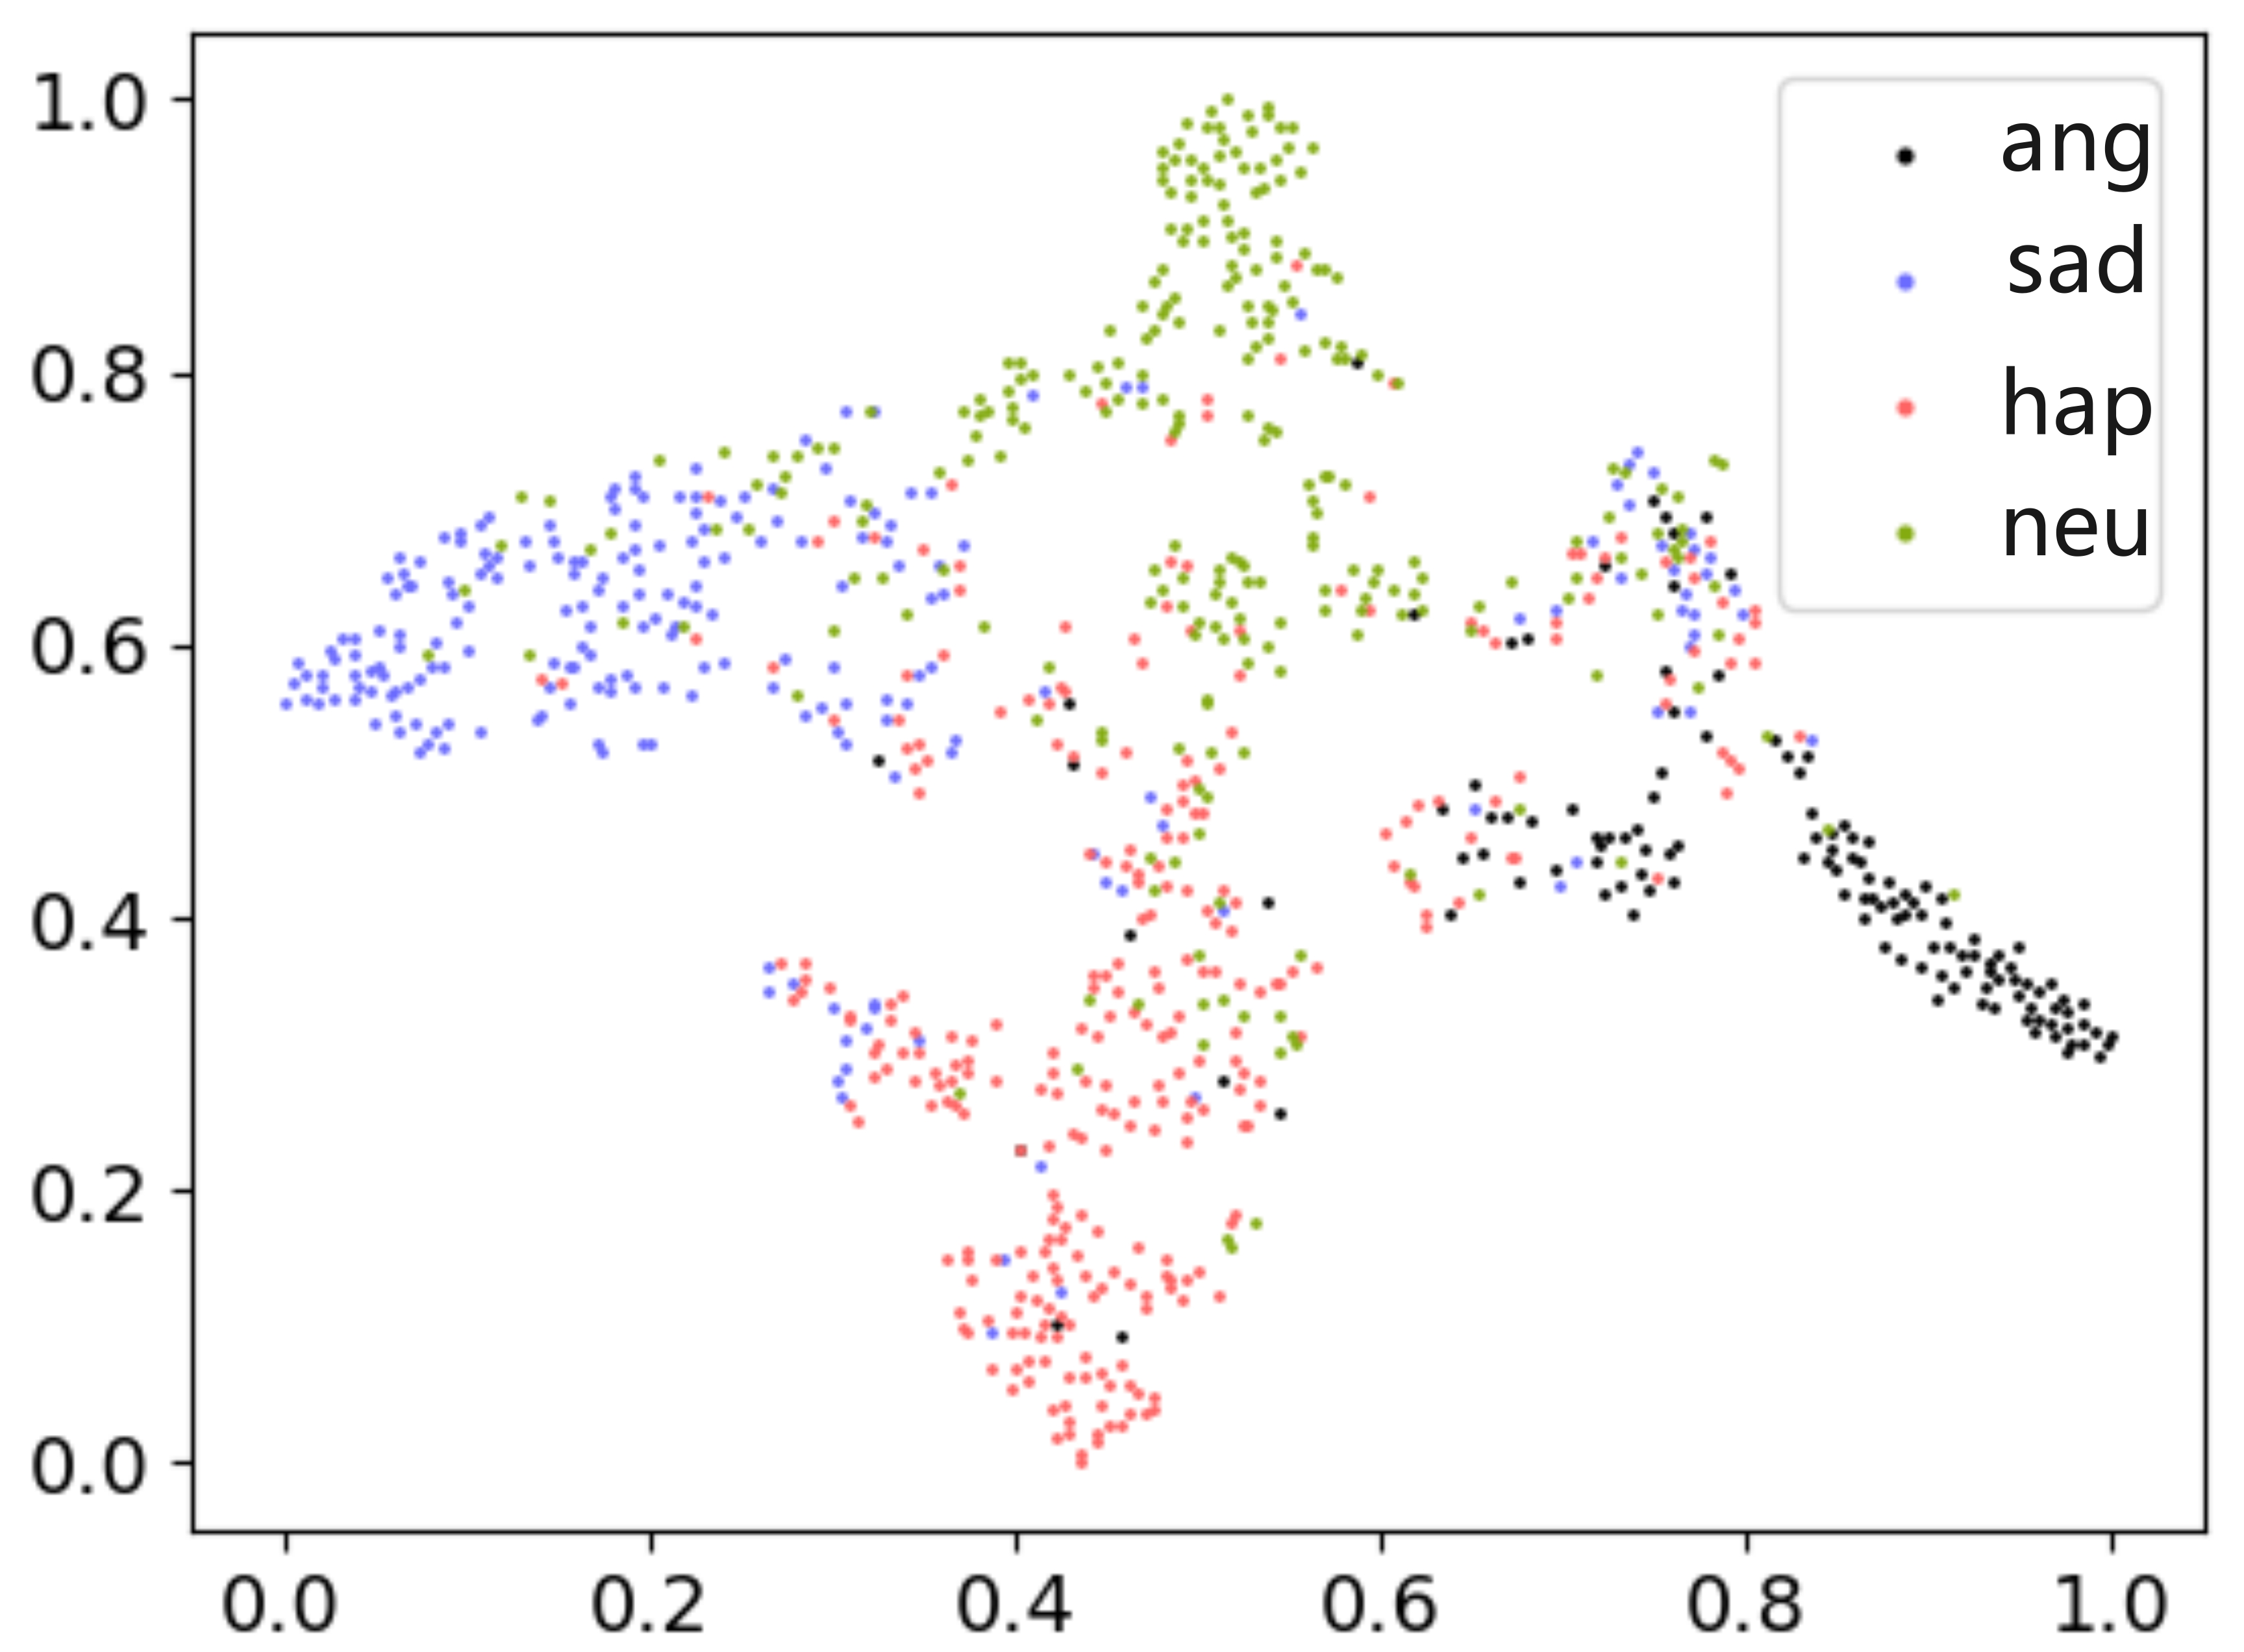
\includegraphics[width=0.8\linewidth]{withCEA_0_2_Fagain.jpg}
    \end{minipage}
}
\caption{The feature distribution visualization using t-SNE. Figure (a) shows the final features without CEA, and Figure (b) shows the final features with CEA.}
\label{TSNE}
\end{figure}


\begin{table}[h]
\centering
\caption{Ablation Study on Network Components.} % 添加标题
\label{Network Components} % 设置标签
\begin{tabular}{l|c|c|cc} 
\hline % 一条横线
\textbf{Models} & \textbf{Wavelet} & \textbf{CEA} & \textbf{WA}(\%) & \textbf{UA}(\%) \\
\hline % 一条横线
\multirow{2}*{EfficientNet + LSTM + wav2vec2} & \XSolidBrush & \XSolidBrush & 70.22 & 71.02 \\
\cline{2-3} % 为第二列到第三列添加横线
& \Checkmark & \XSolidBrush & 69.50 & 71.28 \\ % 第二行需要显示的数据
\hline % 一条横线
\multirow{2}*{EfficientNet + LSTM + WavLM} & \XSolidBrush & \XSolidBrush & 72.99 & 72.88 \\
\cline{2-3} % 为第二列到第三列添加横线
& \Checkmark & \XSolidBrush & 74.17 & 74.96 \\ % 第二行需要显示的数据
\hline % 一条横线
\multirow{2}*{EfficientNet + WavLM} & \XSolidBrush & \XSolidBrush & 73.72 & 74.49 \\
\cline{2-3} % 为第二列到第三列添加横线
& \XSolidBrush & \Checkmark & 74.76 & 75.09 \\ % 第二行需要显示的数据
\hline % 一条横线
\multirow{2}*{Mamba + WavLM} & \XSolidBrush & \XSolidBrush & 73.49 & 74.40 \\
\cline{2-3} % 为第二列到第三列添加横线
& \XSolidBrush & \Checkmark & 75.27 & 76.47 \\ % 第二行需要显示的数据
\hline % 一条横线
\multirow{4}*{EfficientNet + Mamba + WavLM} & \XSolidBrush & \XSolidBrush & 74.10 & 75.45 \\
\cline{2-3} % 为第二列到第三列添加横线
& \Checkmark & \XSolidBrush & 73.69 & 74.28 \\ % 第二行需要显示的数据
\cline{2-3} % 为第二列到第三列添加横线
& \XSolidBrush & \Checkmark & 74.84 & 75.74 \\ % 第二行需要显示的数据
\cline{2-3} % 为第二列到第三列添加横线
& \Checkmark & \Checkmark & \textbf{76.60} & \textbf{77.41} \\ % 第二行需要显示的数据
\hline % 一条横线
\end{tabular}
% 标题和标签写在这里也可以
\end{table}

%\begin{table}[h]
%\centering
%\caption{Ablation experiment on Mamba hidden layer dimension.} % 添加标题
%\label{mamba_exp} % 设置标签
%\begin{tabular}{l c|c c c c c} 
%\hline % 一条横线
%\textbf{Dimension} & & \textbf{WA}(\%) & & & &\textbf{UA}(\%) \\
%\hline % 一条横线
%32  & & 67.98 & & & & 68.37 \\
%64 & & 76.60  & & & &  77.41 \\
%128 & & 72.94 & & & &  73.59 \\
%\hline % 一条横线
%\end{tabular}
% 标题和标签写在这里也可以
%\end{table}

\begin{figure}[htbp]
\centering
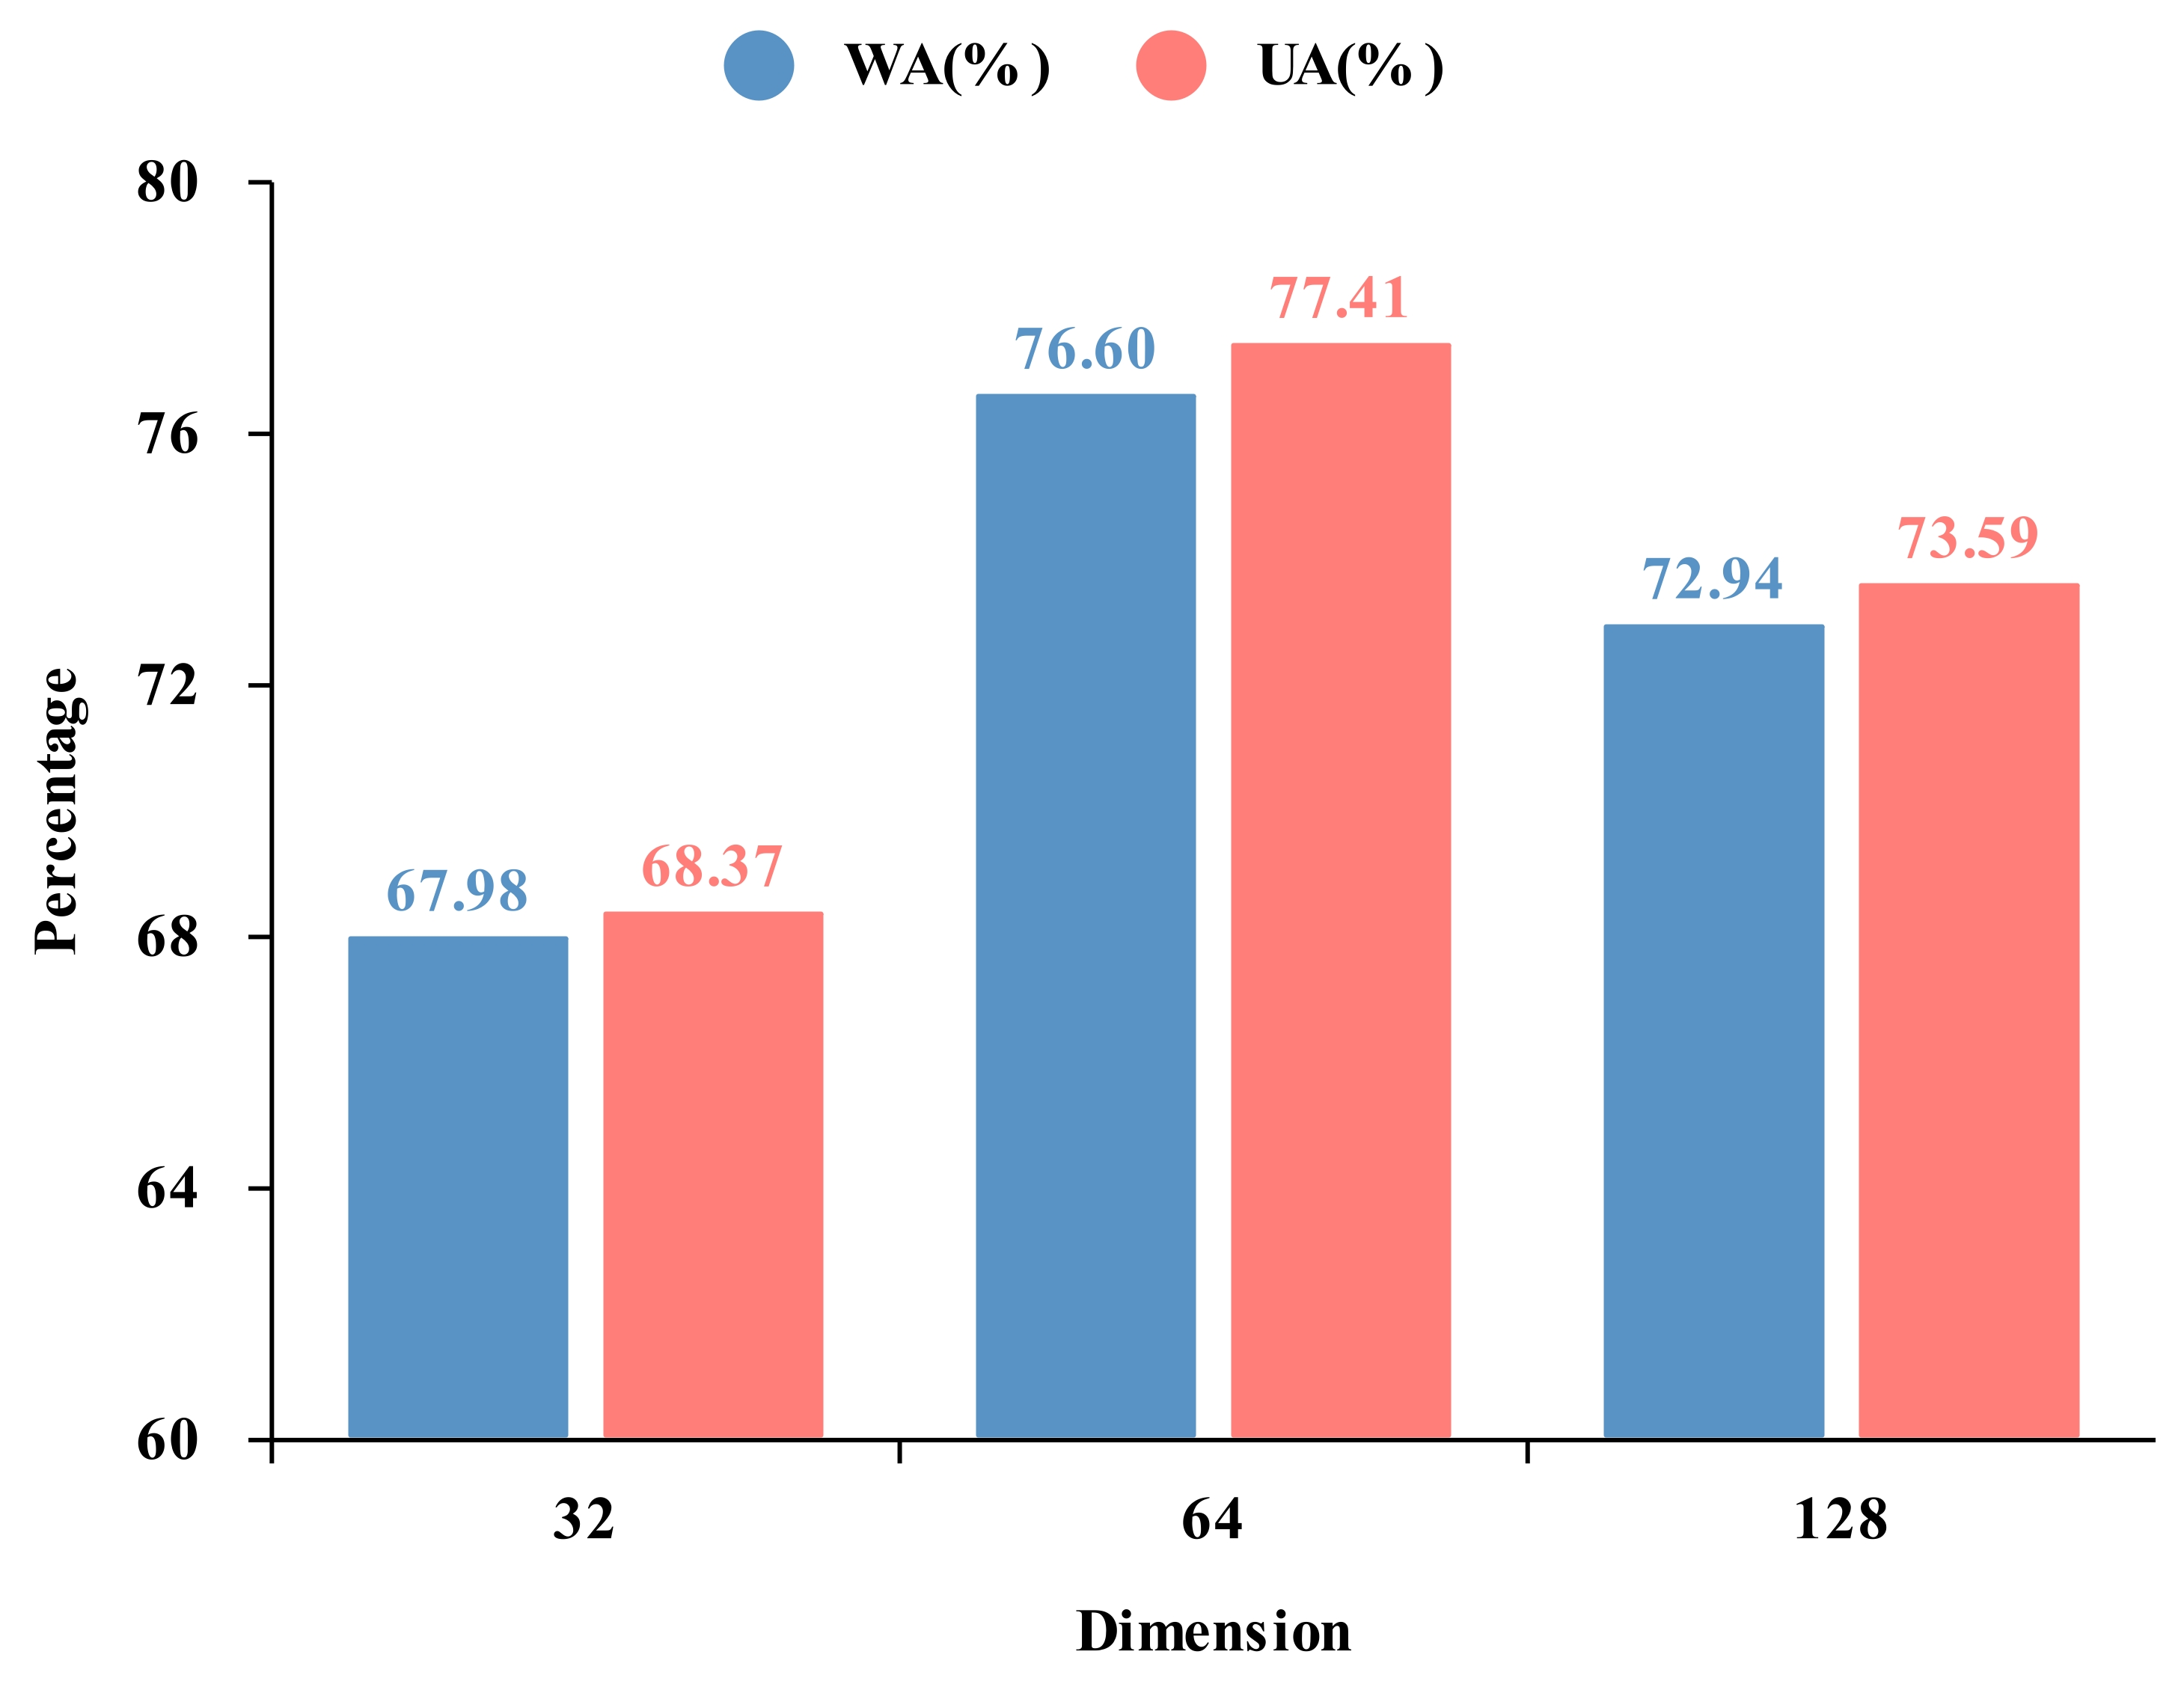
\includegraphics[width=0.9\linewidth]{mamba_dimension.jpg}
\caption{Ablation experiment on Mamba hidden layer dimension}
\label{mamba_exp}
\end{figure}

\begin{figure}[htbp]
\centering
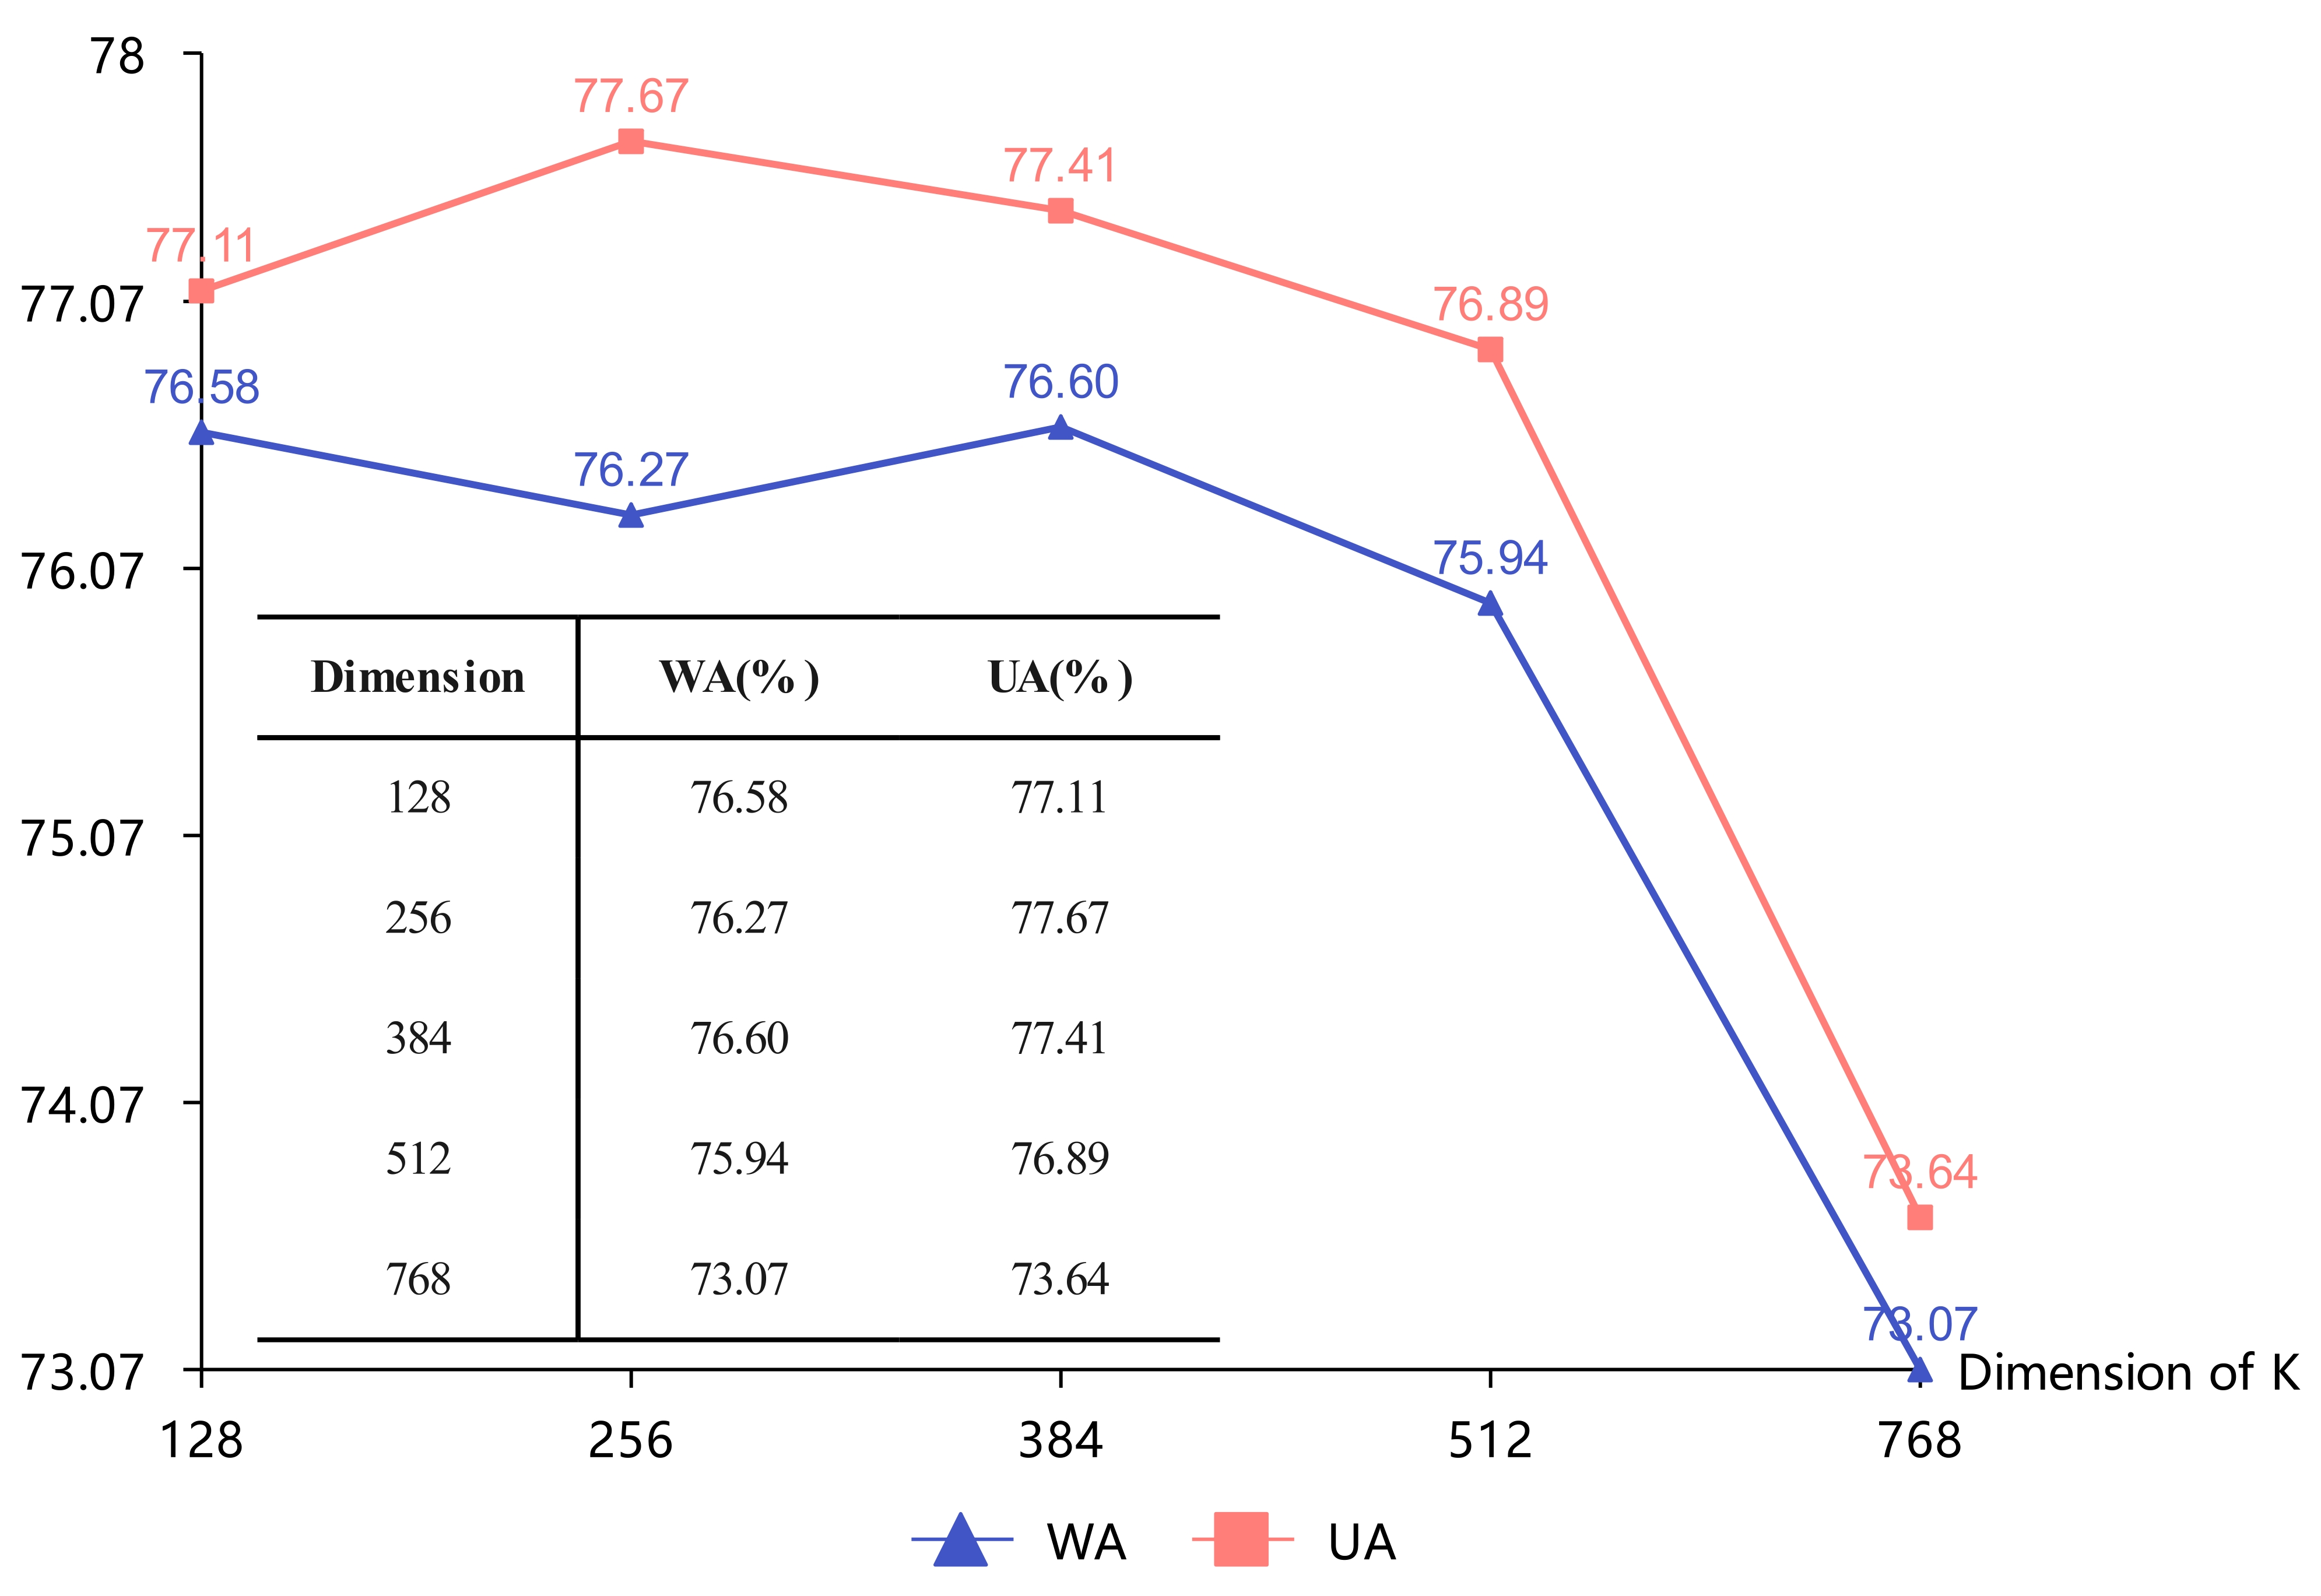
\includegraphics[width=1.\linewidth]{line_322.jpg}
\caption{The changing trend of WA and UA with the dimension change of K}
\label{line}
\end{figure}

The results of our ablation experiments are shown in Table \ref{Network Components}, which fully demonstrate the effectiveness of the proposed method. In the table, EfficientNet represents the log-spectrogram features, Mamba represents the MFCC features, and WavLM represents the WLM features. In the experiments without CEA, we only use the co-attention mechanism to ensure comparability.  The first two rows and the last four rows in the table present the results of different feature extraction module combinations. By comparing these three combinations, it can be observed that the Mamba module and WavLM model help improve emotion recognition performance. By comparing the emotion recognition accuracy with and without wavelet transform on the log-spectrogram features, the results indicate that the wavelet transform can slightly improve the emotion recognition accuracy. In row 12 of Table \ref{Network Components}, the accuracy slightly decreases when the wavelet transform is applied, possibly because the co-attention mechanism is not particularly suitable for processing features extracted from wavelet-transformed spectrograms. The following two rows present the combinations of WLM with log-spectrogram and MFCC features and compare the results with or without CEA. From the comparison, it can be observed that CEA can effectively utilize the cooperation between other acoustic information and WLM, resulting in approximately a 1\% improvement in recognition accuracy for both types of acoustic information. From the last four rows, it can be seen that the CEA module effectively focuses on the emotion-related information in WLM and better integrates the three features, improving emotion recognition accuracy. Figure \ref{mamba_exp} shows the impact of changes in the hidden layer dimension of Mamba on model performance. It can be seen that when the hidden layer dimension of Mamba is set to 64, the model achieves optimal performance. Figure \ref{line} illustrates the effect of changes in the dimension \( K \) on the performance of CEA. It can be observed that the best experimental results are obtained when \( K \) is set to 384.

Figure \ref{TSNE} shows the feature distribution with and without CEA, visualized using t-SNE. It can be seen that after applying CEA, points of the same class are more tightly clustered, and the decision boundaries of the features are clearer.

\section{CONCLUSION}
This paper presents a novel SER method that utilizes CEA for the collaboration and enhancement of multiple acoustic features. In this method, we apply wavelet transform to convert the raw audio into the frequency domain and use multiple feature extraction modules, such as Mamba, to extract features from different acoustic information. Furthermore, CEA facilitates the collaboration between the spectrogram, MFCC, and WLM, enhancing the emotional information in the WavLM features. Experimental results on the IEMOCAP dataset demonstrate the effectiveness of our approach.
%
% ---- Bibliography ----
%
% BibTeX users should specify bibliography style 'splncs04'.
% References will then be sorted and formatted in the correct style.
%
% \bibliographystyle{splncs04}
 \bibliographystyle{unsrt}
 \bibliography{ref}
%
%\begin{thebibliography}{8}
%\bibitem{ref_article1}
%Author, F.: Article title. Journal \textbf{2}(5), 99--110 (2016)

%\bibitem{ref_lncs1}
%Author, F., Author, S.: Title of a proceedings paper. In: Editor,
%F., Editor, S. (eds.) CONFERENCE 2016, LNCS, vol. 9999, pp. 1--13.
%Springer, Heidelberg (2016). \doi{10.10007/1234567890}

%\bibitem{ref_book1}
%Author, F., Author, S., Author, T.: Book title. 2nd edn. Publisher,
%Location (1999)

%\bibitem{ref_proc1}
%Author, A.-B.: Contribution title. In: 9th International Proceedings
%on Proceedings, pp. 1--2. Publisher, Location (2010)

%\bibitem{ref_url1}
%LNCS Homepage, \url{http://www.springer.com/lncs}, last accessed 2023/10/25
%\end{thebibliography}
\end{document}
